\chapter{Networks with Relays}
\begin{quote}
In this chapter, we extend the dynamic program of Chapter 4 for solving the $\ACONN$ problem on partial $k$-trees to solve the $\ARCONN$ and $\SRCONN$ problems. For each problem, we present the modifications required, analyze the running time, and present simulation results to explore some performance and usage aspects.
\end{quote}


\section{Overview of the Extensions}
\label{sec:overviewExt}
Throughout this chapter, the UWSN is modelled by a probabilistic graph $G=(V=V_{sense}\cup V_{relay}$ $,E_G,Loc,p)$ where $V=V_{sense}\cup V_{relay}$, and $V_{relay}$ may contain zero or more relay nodes. As in Chapter 4, we assume that $G$ has the topology of a partial $k$-tree for some specified $k$. In addition, when no confusion arises, we use $G$ to refer also to the partial $k$-tree graph underlying the structure of the probabilistic graph $G$.

%
Our proposed extended algorithm for solving the $\ARCONN$ and  $\SRCONN$ problems have the same structure and organization as the algorithm presented in Chapter 4.
%
Functions Main and $t\_merge$ (but not $p\_merge$) are modified, but maintain their high level structure and steps.
As discussed below, the main modifications concern the formulation of new network state types to solve each problem. The modifications introduce new steps to initialize and maintain the new state types, as well as extract a final solution from them.

\section{The $\ARCONN$ Algorithm}
\label{sec:arconnalg}
We present below the needed modifications to solve the $\ARCONN$ problem.
\subsection{$\ARCONN$ State Types}
\begin{definition}[\textbf{state types of the $\ARCONN$ problem}]\label{def:arconnstatety}
\normalfont
Let $G_{v_i,\alpha}$ be a subgraph reduced onto clique $K_{v_i,\alpha}$. Denote by $V_{v_i,\alpha}$ the set of nodes of the graph $G_{v_i,\alpha}$. Let $S=\{v_a[i_a] :v_a\in V_{v_i,\alpha} \mbox{ and } i_a \in Loc(v_a)\}$  be a network state of $G_{v_i,\alpha}$. \\Then\\
\centerline{
$AR\mbox{-}type(S)=\{V_{1,b(V_1)}^{Loc(V_1)}, V_{2,b(V_2)}^{Loc(V_2)}, \ldots, V^{Loc(V_r)}_{r,b(V_r)} \}$}

where
\begin{itemize}[noitemsep]
\item $\{V_1^{Loc(V_1)}, V_2^{Loc(V_2)}, \ldots, V_r^{Loc(V_r)}\}=A\mbox{-}type(S)$
\item For each part $V_i\subseteq V_{v_i,\alpha}$ of the partition $(V_1,V_2,\ldots,V_r)$, $b(V_i)$ is a binary $(0/1)$ indicator. To explain the setting of $b(V_i)$, let us denote by $S_i \subseteq S$ the connected component of state $S$ that contains all nodes in $V_i$. We set $b(V_i)=1$ if $S_i$ contains at least one sensor node from $V_{sense}$. Else (if $S_i$ is composed of relay nodes only), then $b(V_i)=0$.
 $\blacksquare$
\end{itemize}
\end{definition}

\begin{example}
\normalfont
In figure \ref{fig:sttype1}, denote by $G_{v_i,1}$, the graph induced on nodes $\{v_a,v_b,v_i,v_j,v_k\}$. Assume that $\{v_b\}\in V_{sense}$ and $\{v_a,v_i,v_j,v_k\} \in V_{relay}$. Suppose that state $S$ of figure \ref{fig:sttype1_node} is a possible network state of $G_{v_i,1}$. Then $AR\mbox{-}type(S)=\big \{\{v_i\}_1^{(1)},\{v_j,v_k\}_0^{(2,3)}\big\}$. Here, the indicator $b(\{v_i\})=1$ since $v_b$ is a sensor node connected to $v_i$ in $S$. $\blacksquare$
\end{example}
\begin{figure}[!htb]
\begin{minipage}[]{0.5\linewidth}
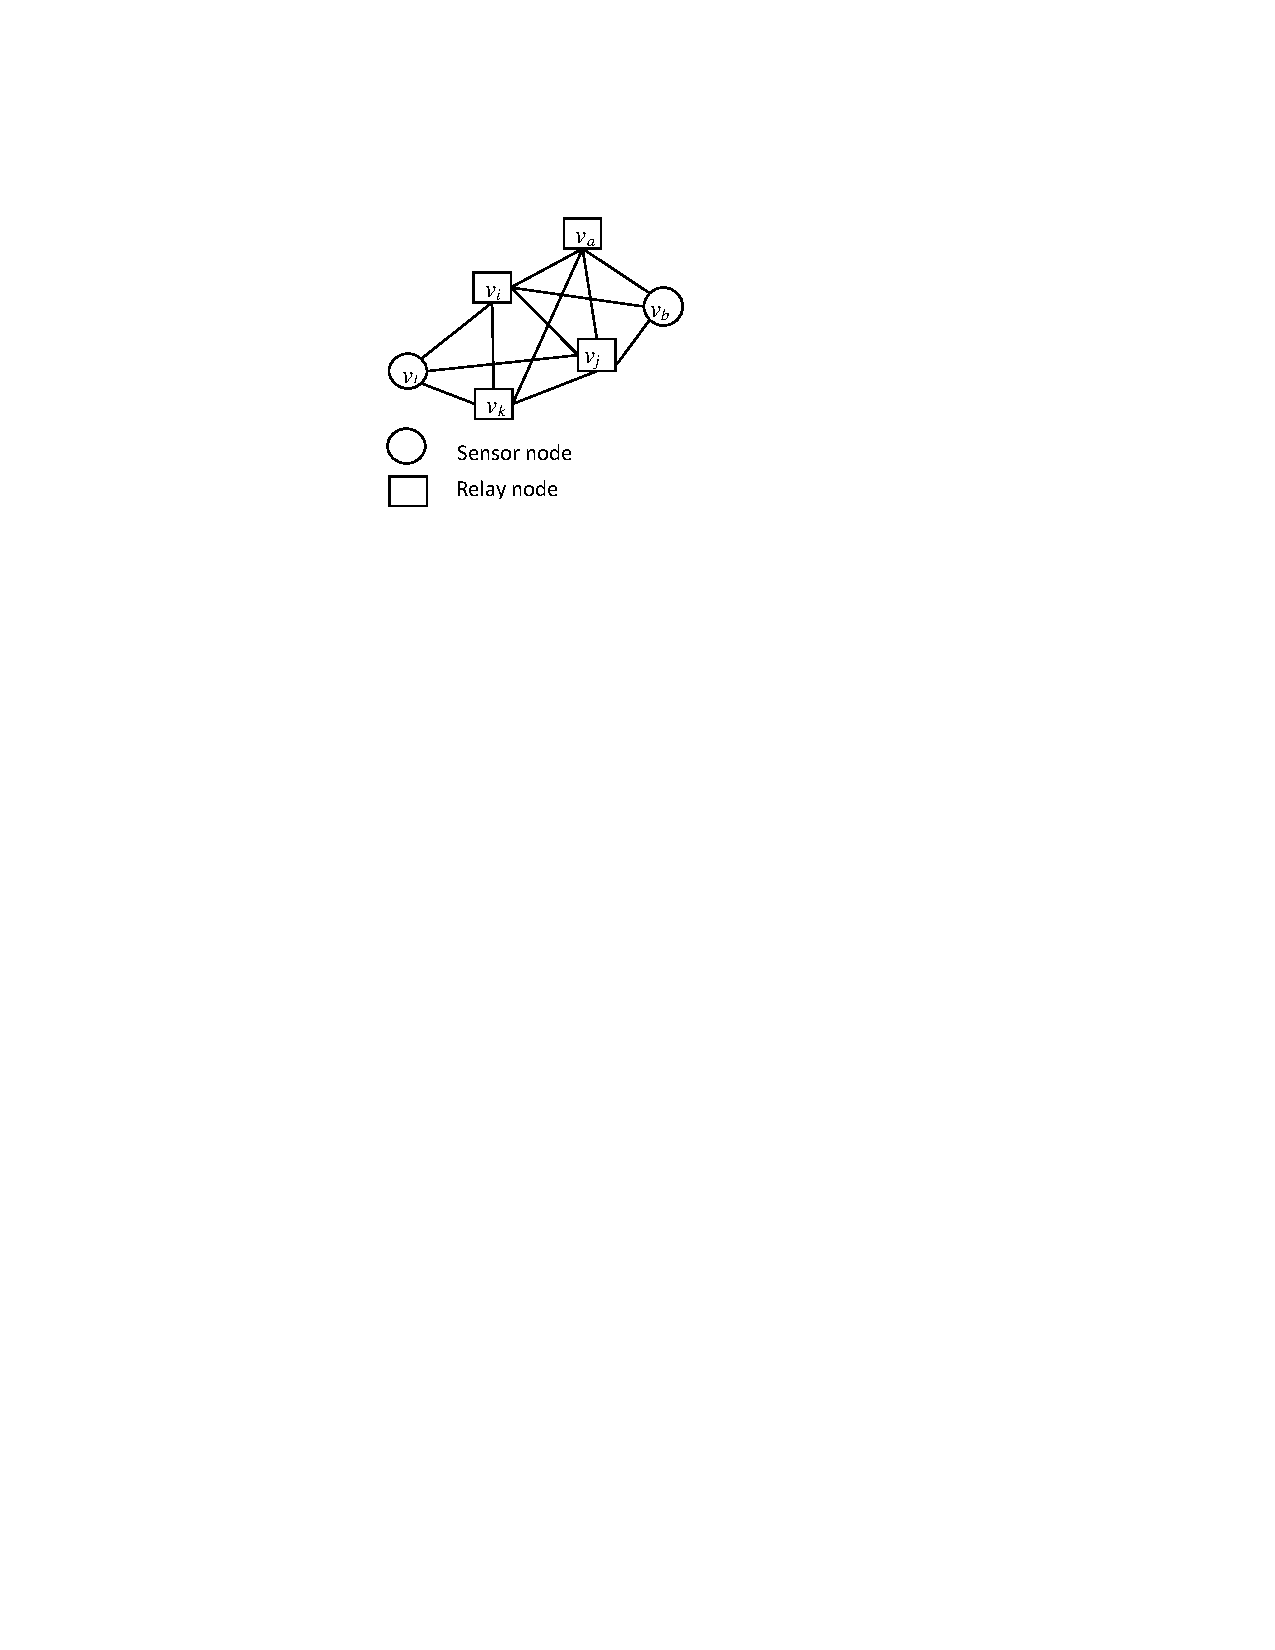
\includegraphics[width=2.2 in, height=1.8 in]{Ch5f2.pdf}
\caption{A fragment of a 3-tree}
\label{fig:sttype1}
\end{minipage}
\begin{minipage}{0.5\linewidth}
\nwline
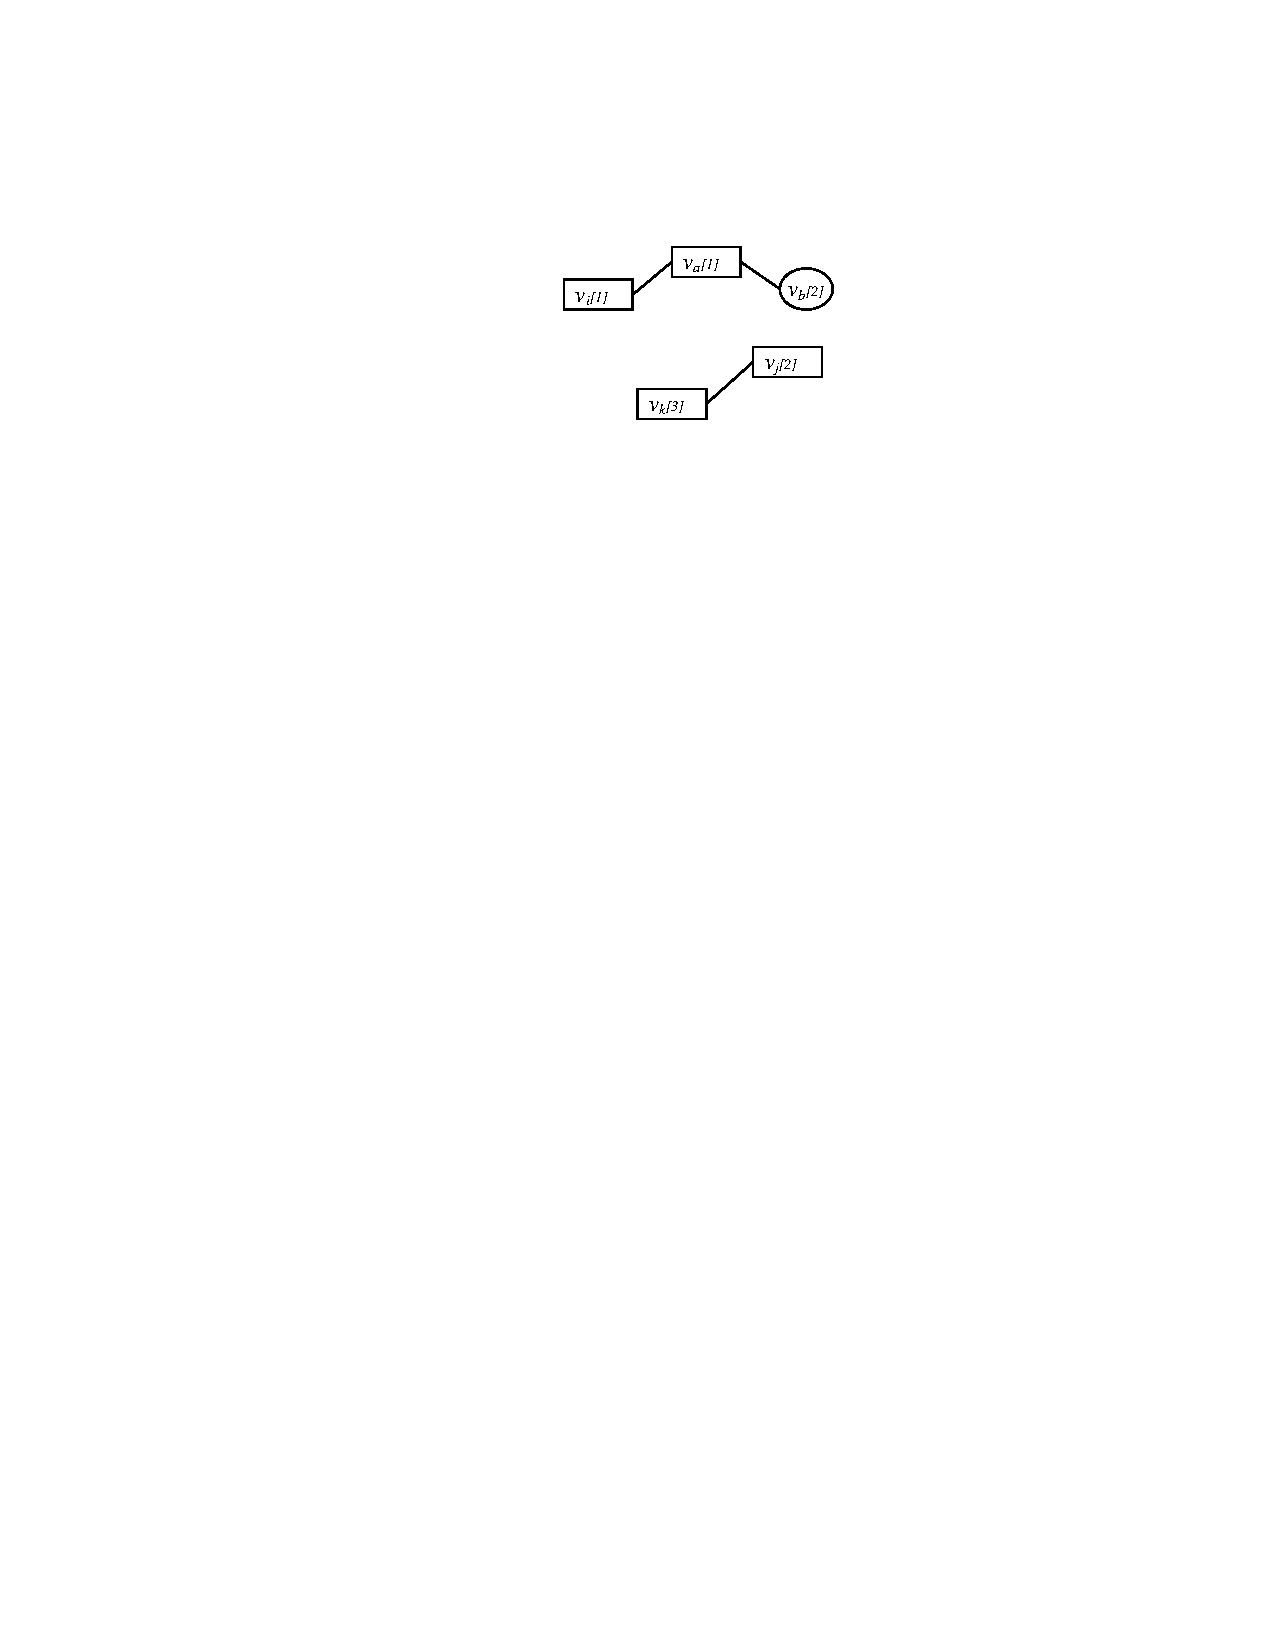
\includegraphics[width=1.7 in, height=1.5 in]{Ch5f2_1.pdf}
\caption{A state $S$ on $\{v_a,v_b,v_i,v_j,v_k\}$}
\label{fig:sttype1_node}
\end{minipage}
\end{figure}
The rationale behind the definition of $AR\mbox{-}types$ is that when we merge tables containing information of two subgraphs $G_{v_i,1}$ and $G_{v_i,2}$ to compute summary information of the union graph $G_{v_i,1}\cup G_{v_i,2}$, we need to know which connected components contain at least one sensor node (and thus, are essential to form an operating state), or contain relay nodes only (and thus, may not be essential to form an operating state). 
\subsection{Initializing Tables}
\label{subsec:initt}
Step 1 of function Main initializes a table $T_H$ associates with each $k$-cliques $H$ of the full graph $k$-tree($\tilde{G}$).
Similar to the approach used in Chapter 4, we perform the following steps,
\begin{enumerate}[noitemsep]

\item We construct for each edge $e=\{x,y\}$ in $H$ an exhaustive table $T_e$ where the keys are of the $AR$-$type$.
\item We use $t\_merge$ and $p\_merge$ to compute the cross product of all tables associated with all edges in the $k$-clique $H$.
\end{enumerate}

\subsection{Merging $\ARCONN$ State Types}
\label{subsec:mst}

We recall that function $t\_merge$ takes as input two table $T_1$ and $T_2$ that may have a set $C=V(T_1)\cap V(T_2)$ of common nodes, and produces a new table $T_{out}$. The context of the merge operation is as follows. 


Each table $T_i, i=1,2,$ contains summary information about a subgraph $G_i$ that has been reduced onto a clique $K_i$. The merge operation computes a table $T_{out}$  that stores summary information about the graph $G_1\cup G_2$.

$T_{out}$ is computed by processing each pair of keys (i.e., $\ARCONN$ state types) $key_1\in T_1$ and $key_2\in T_2$. Processing $key_1 \mbox{ and } key_2$ results in a new state type, denoted $key_{out}$, and an associated probability, denoted $p_{out}$.
%
To explain processing of $key_1$ and $key_2$, consider two network states: $S_i, i=1,2,$ of the subgraph $G_i$ reduced onto the clique $K_i$, where $key_i=AR\mbox{-}type(S_i)$. Merging $S_1$ and $S_2$ generates $key_{out}=AR\mbox{-}type(S_1\cup S_2)$.

As in Chapter 4, such a union is possible only if each common node in $C$ assumes the same position in both of $S_1$ and $S_2$. Else, the two keys are not compatible, and no $key_{out}$ is generated.

To explain the structure of $key_{out}$ (if it exists), let\\
\nwline
\begin{center}
$\begin{array}[t]{l}
AR\mbox{-}type(S_1)=\{X_{i,b(X_i)}^{Loc(X_i)} : i=1,2, \ldots\},\\
AR\mbox{-}type(S_2)=\{Y_{j,b(Y_j)}^{Loc(L_j)} : j=1,2, \ldots\}, and\\
AR\mbox{-}type(S_1\cup S_2)=\{Z_{k,b(Z_k)}^{Loc(Z_k)} : k=1,2, \ldots\}\end{array}$.
\end{center}
Then 
\begin{itemize}[noitemsep]
\item The partition $\{Z_k:k=1,2,\}$ is generated by applying partition merge to $\{X_i:i=1,2,\ldots\}$ and $\{Y_j:j=1,2,\ldots\}$.
\item The binary indicator obtained by merging two parts, say $X_i$ and $Y_j$ is  $max(b(X_i),b(Y_j))$.
\end{itemize}
Similar to the $\ACONN$ algorithm, the probability $p_{out}$ is the product $T_1(key_1) \times T_2(key_2)$ divided by a correction term  $=\prod \big (p_x(i):x[i] \mbox{ is common between } key_1 \mbox{ and } key_2\big)$.

%%%%
%Example 5.6 Same as example 4.6
%

\subsection{Removing Bad State Types}
\label{subsec:rbst}
We recall that the first part of the main loop of function Main merges all tables $\{T_{v_i,\alpha} :\alpha=base,1,2, \ldots,k\}$ into table $T_{v_i,base}$. The second part of the main loop (Steps 7 to 10) removes bad state types from table $T_{v_i,base}$ prior to deleting node $v_i$.
%
For the $\ARCONN$ problem, a state $S$ of the subgraph $G_{v_i,base}$ reduced onto the $k$-clique $K_{v_i,base}$ is considered bad at this stage if node $v_i$ appears as a singleton part in the partition associated with $AR\mbox{-}type(S)$ and the indicator $b({v_i})=1$.


 This badness follows since $S$ has a connected component with at least one sensor node, and this component reaches outside nodes via node $v_i$, yet node $v_i$ is disconnected from other nodes in $K_{v_i,base}$. The algorithm removes all such bad state types from $T_{v_i,base}$.

Else if $AR\mbox{-}types(S)$ is good then one of the following cases applies:
\begin{itemize}[noitemsep]
\item \textbf{Case: $v_i$ is a singleton part and $b(\{v_i\})=0$}. Here, the part $\{v_i\}$ is merely removed from $AR\mbox{-}type(S)$.
\item \textbf{Case: $v_i$ is not singleton}. Assume that $v_i$ belong to part $V_1$, where $|V_1|\geq 2$. Then node $v_i$ and its associated position is removed from $V_1$.
\end{itemize}

\subsection{Obtaining Final Result}
\label{subsec:ofr}
Step 11 of function Main is modified to compute $Conn(G)$ as the sum of all values in table $T_{v_{n-k},base}$ corresponding to $AR\mbox{-}types$ of the form\\
\nwline
\centerline{
$\{X_{i,b(X_i)}^{Loc(X_i)} : i=1,2, \ldots\}$}
where
\begin{itemize}[noitemsep]
\item the particular part of the partition ${X_1,X_2,\ldots,X_r}$ that contains the sink node, say $X_1$, has $b(X_1)=1$, and 
\item each other part $X_j, j \neq 1,$ of the partition has $b(X_j)=0$.
\end{itemize}
That is, step 11 considers only network states where any connected component disconnected from the sink does not have any sensor node. Thus, all sensor nodes must lie in the same component of the sink node.

\subsection{Running Time}
\label{subsec:rt}

As in Chapter 4, $n$ denotes the number of nodes in $G$, $l_{max}$ denotes the maximum number of locations in the locality set of any node, and $B_k$ denote the $k^{th}$ Bell number.
\begin{theorem}\normalfont In the $\ARCONN$ algorithm we have\label{thm:rt}
\begin{enumerate}[noitemsep]
\item The maximum length of any table is $O(B_kl_{max}^k2^k)$ 
\item The worst case running time is $O(n(B_kl_{max}^k2^k)^2)$
\end{enumerate}
\end{theorem}


The proof is similar to the proof of the Theorem \ref{thm:runtym} by observing that adding indicator bits to state types makes the maximum table length as specified in part 1.
\section{$\ARCONN$ Simulation Results}
\label{sec:arconnsim}
Relay nodes are expected to be cheaper than sensor nodes since they do not include sensing devices. In addition, relay nodes are not required to do energy consuming data acquisition tasks as sensor nodes. Hence, their design may enjoy more flexibility than sensor nodes, and their energy supply is expected to last longer.

In this section we utilize the algorithm developed for the $\ARCONN$ problem to investigate the positive effects of deploying relay nodes.
\begin{figure}[!htb]
\begin{minipage}{.9\linewidth}
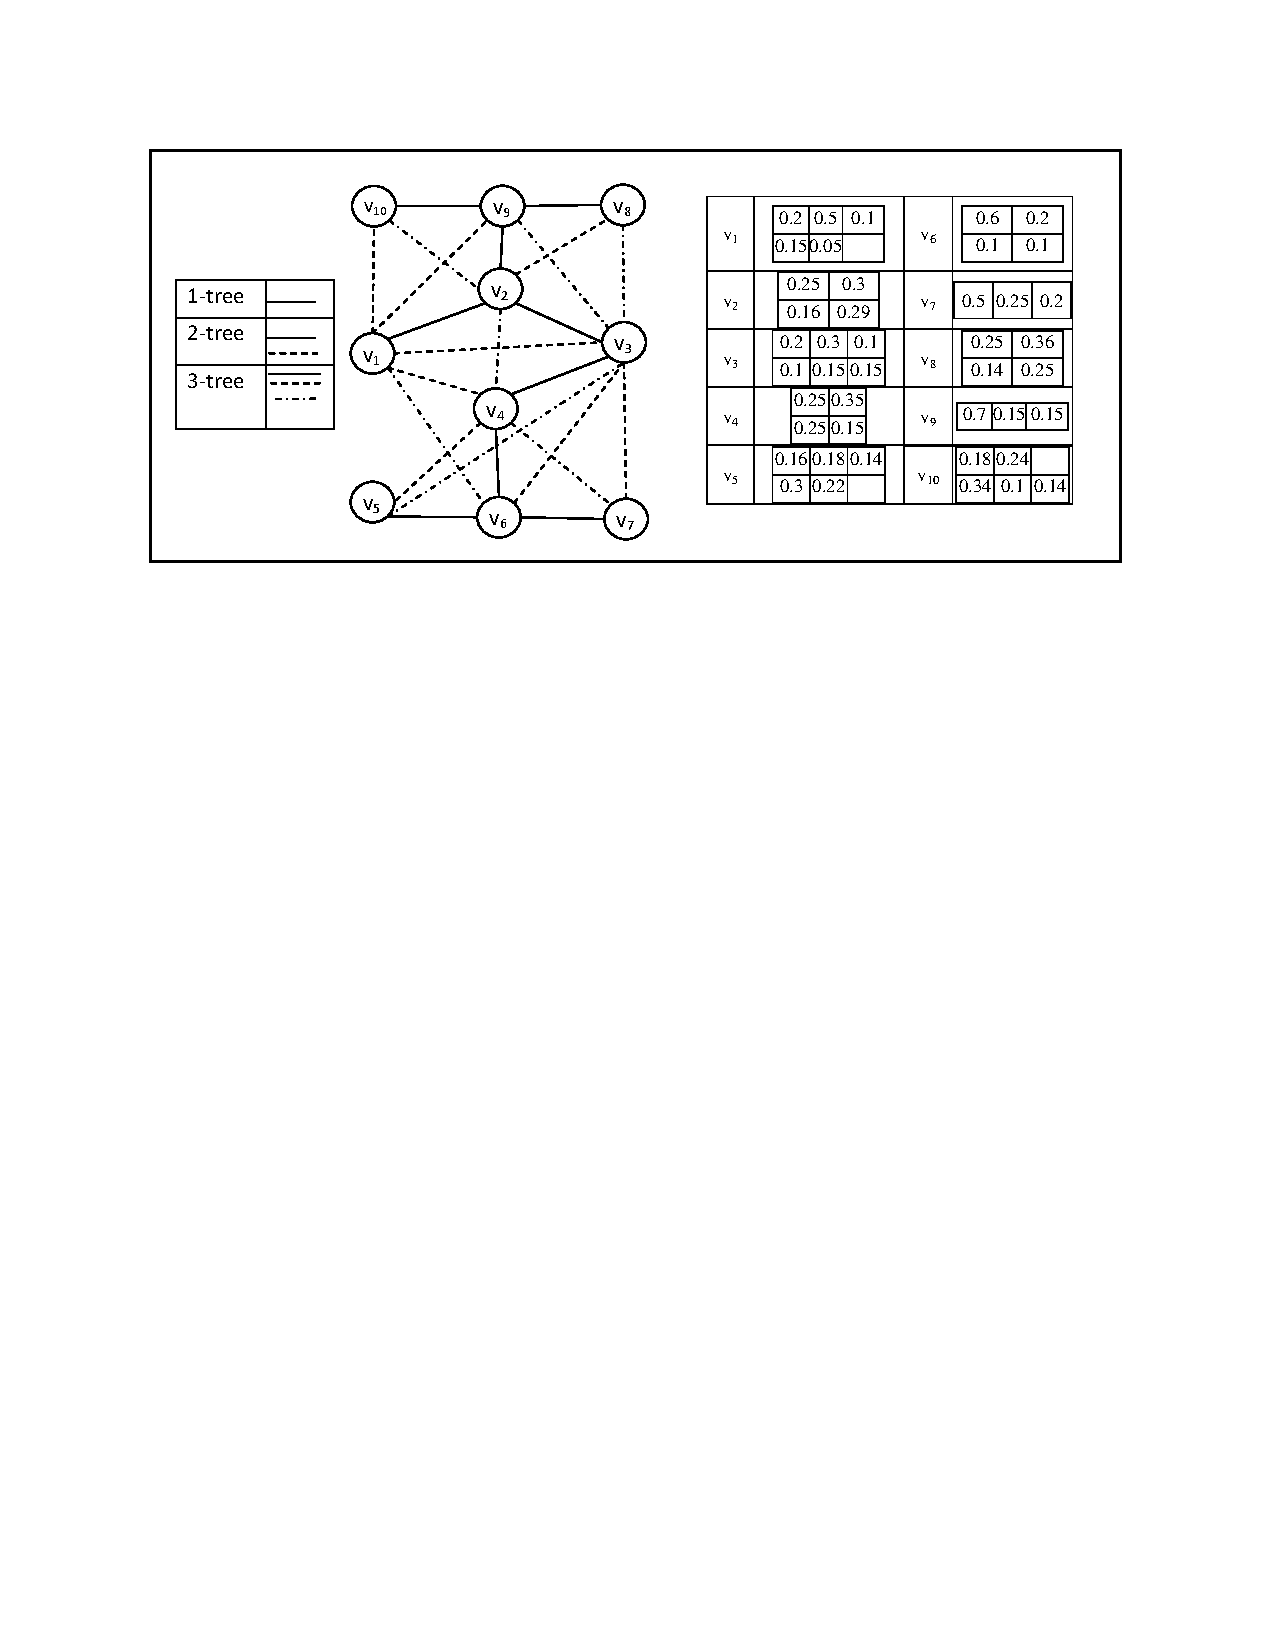
\includegraphics[width=6 in, height=2.8 in]{NetworkI_paper.pdf}
\caption{Network $G_{10}$}
\label{fig:netI1}
\end{minipage}
\end{figure}

\begin{figure}[!htb]
\begin{minipage}{.9\linewidth}
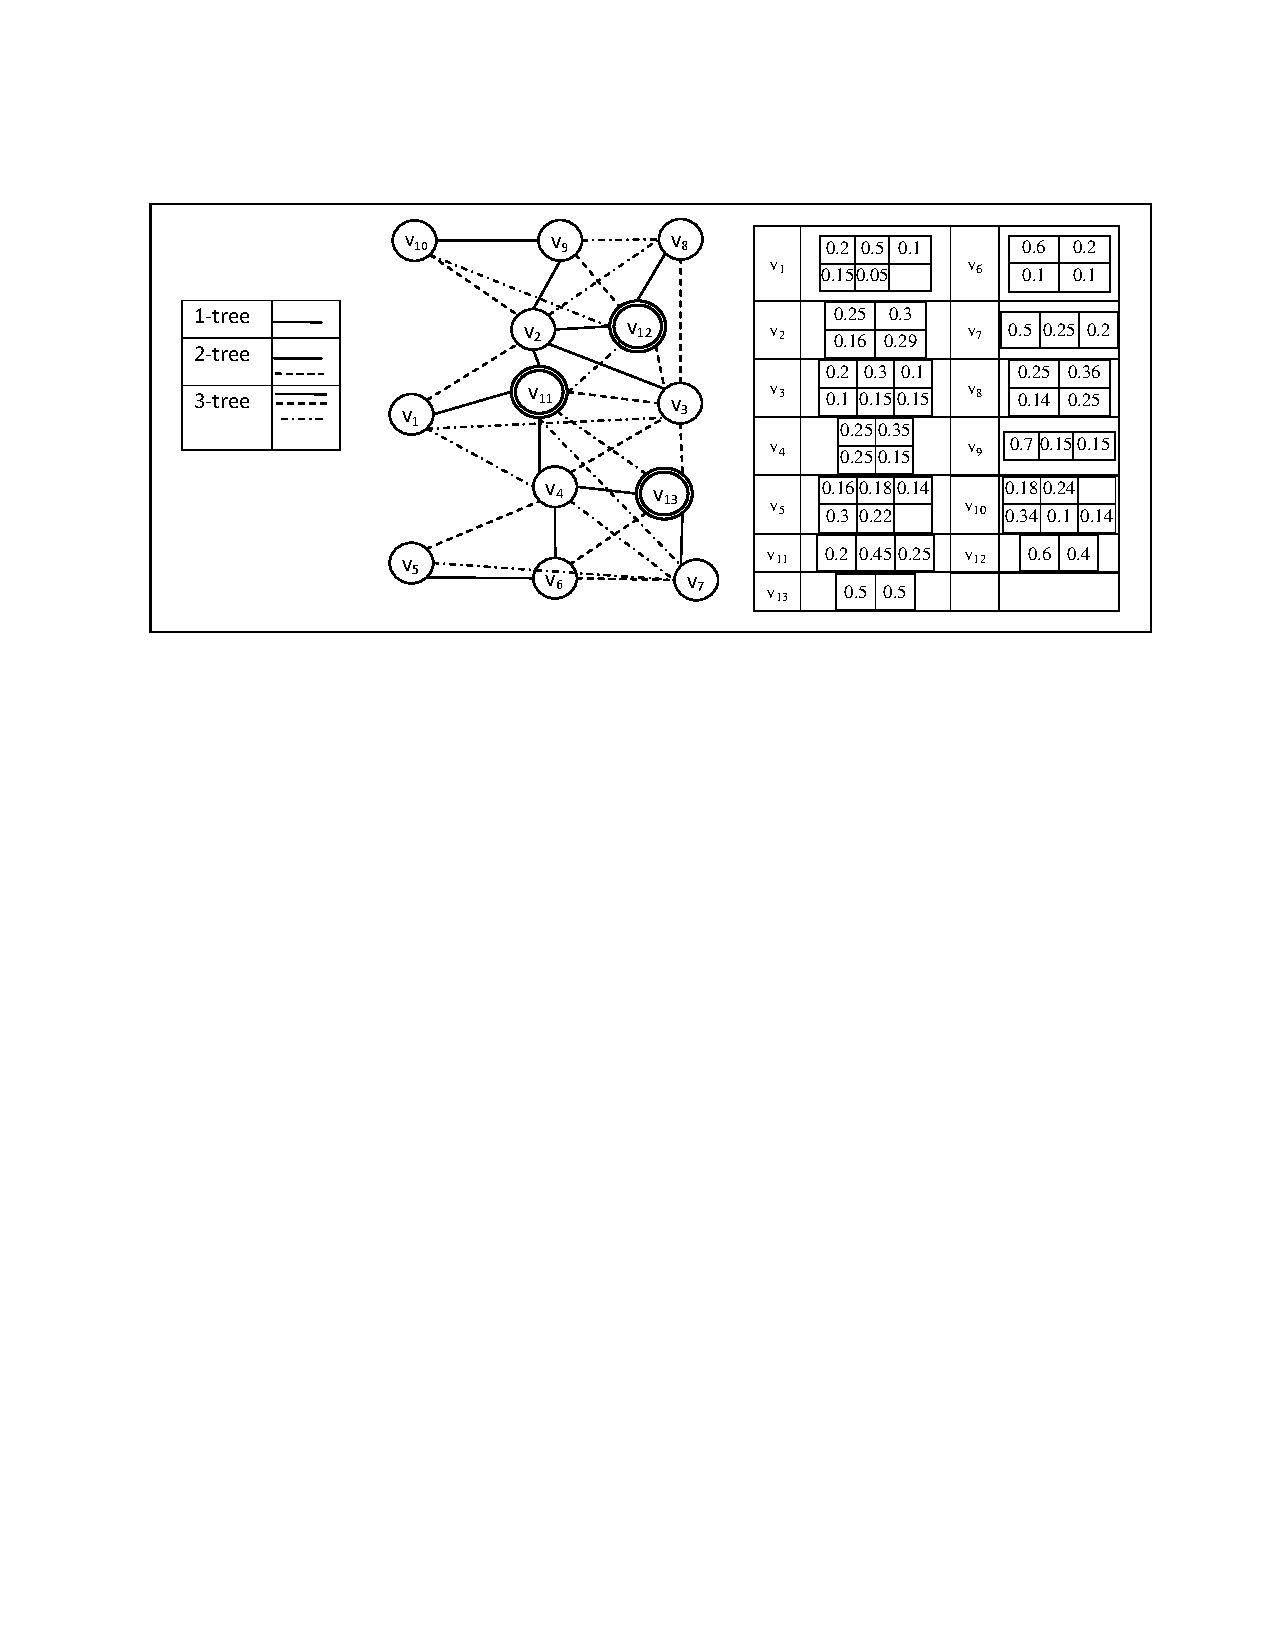
\includegraphics[width=6 in, height=2.8 in]{NetworkI_paper_Relay.pdf}
\caption{Network $G_{10,3}$}
\label{fig:netIR}
\end{minipage}
\end{figure}

\textbf{Test Networks:} To illustrate our basic findings, we present results on network $G_{10}$ (figure \ref{fig:netI1}) and network $G_{10,3}$ (figure \ref{fig:netIR}) which adds 3 relay nodes to $G_{10}$. In each network, $v_1$ is the sink node, and all edges shown in the figures appear when $R_{tr}\geq 6.5$ units. Reducing $R_{tr}$ results in networks with possibly fewer edges. We experiment with a tree, 2-tree, and 3-tree subgraphs shown by the solid and dotted lines in the figure. The subgraphs are obtained using the greedy method of Chapter 2.

\begin{enumerate}
\item \textbf{Running Time:} Table \ref{Tab:rtym1} shows the increase of running time as the dynamic program moves from using $A\mbox{-}type$ keys on $G_{10}$ to using $AR\mbox{-}type$ keys on $G_{10,3}$ 
\begin{table}[!htb]
    %\caption{Global caption}
    \begin{minipage}{1\linewidth}
   
      \centering
     \begin{tabular}{|c|c|c|}
     \hline
         k& Network $G_{10}$ &Network $G_{10,3}$\\
     \hline
     1&90& 110 \\\hline
     2&1000 &6000	\\\hline
3 &6000&8000	 \\\hline
\end{tabular}
 \caption{Running time in milliseconds}
\label{Tab:rtym1}
    \end{minipage}
\end{table}
\item \textbf{Effect of adding relay nodes:} Table \ref{Tab:SRC} shows the obtained bounds on $G_{10}$ and $G_{10,3}$. As can be seen, adding 3 relay nodes can enhance the computed $Conn(G)$ by, e.g. $63\%$ (the $3^{rd}$ row).


\begin{table}[!htb]
  \centering
 \begin{minipage}{.5\linewidth}
     \begin{tabular}{|c|c|c|}
     \hline
     k & Network $G_{10}$ & Network $G_{10,3}$  \\
     \hline
      1 & 0.30 & 0.86 \\\hline
	  2 & 0.54 & 0.96\\\hline
	  3 &0.60 & 0.98 \\\hline
\end{tabular}
    \end{minipage}
     \caption{Connectivity with respect to $k$}
      \label{Tab:SRC}   
\end{table}
\item \textbf{Effect of adding relay nodes for various node $R_{tr}$:}
Figure \ref{Fig:NWOR} illustrates $Conn(G)$, on  $G_{10}$ and $G_{10,3}$ as $R_{tr}$ varies in the range $[2.5,7.5]$. Each obtained curve exhibits a notable monotonic increasing behaviour as $R_{tr}$ increases. As explained in Chapter 4, this behaviour is due to the appearance of more edges as $R_{tr}$ increases, and the potential increase in the probability of each edge as $R_{tr}$ increases. Increasing $R_{tr}$, however, requires increasing node energy consumption. To achieve a desired $Conn(G)$ value, a designer may utilize the obtained curves to assess the merit of increasing $R_{tr}$ versus deploying more relay nodes.
\begin{figure}[!htb]
\begin{minipage}{.9\linewidth}
\end{minipage}
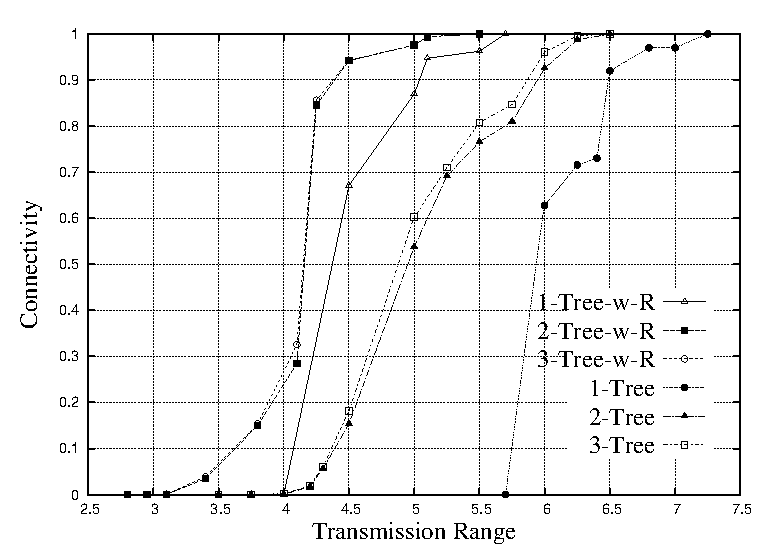
\includegraphics[width=6 in, height=2.6 in]{NetworkI_woR.eps}
\caption{Connectivity versus transmission range}
\label{Fig:NWOR}
\end{figure}

\end{enumerate}






\section{The $\SRCONN$ Algorithm}
\label{sec:sralg}
Next, we present the needed modifications to solve the $\SRCONN$ problem.
\subsection{$\SRCONN$ State Types}
\label{subsec:srst}

\begin{definition}[\textbf{state types of the $\SRCONN$ problem}]\label{def:srst}
Let $G_{v_i,\alpha}$ be a subgraph reduced onto a clique $K_{v_i,\alpha}$. Denote by $V_{v_i,\alpha}$ the set of nodes of the graph $G_{v_i,\alpha}$. Let $S=\{v_a[i_a] :v_a\in V_{v_i,\alpha} \mbox{ and } i_a \in Loc(v_a)\}$  be a network state of $G_{v_i,\alpha}$.\\
Then
\nwline
\centerline{
$SR\mbox{-}type(S)=\{V_{1,c(V_1)}^{Loc(V_1)}, V_{2,c(V_2}^{Loc(V_2)}, \ldots, V^{Loc(V_r)}_{r,c(V_r} \}$}

where
\begin{itemize}[noitemsep]
\item $\{V_1^{Loc(V_1)}, V_2^{Loc(V_2)}, \ldots, V_r^{Loc(V_r)}\}=A\mbox{-}type(S)$
\item For each part $V_i\subseteq V_{v_i,\alpha}$ of partition $(V_1,V_2,\ldots,V_r)$, $c(V_i)$ is the number of sensor nodes in the connected component $S_i \subseteq S$  that includes all nodes in $V_i$.
 $\blacksquare$
\end{itemize}
\end{definition}

\begin{example}
\normalfont
 In figure \ref{fig:sttype2}, denote by  $G_{v_i,1}$, the graph induced on nodes $\{v_a,v_b,v_i,v_j,v_k\}$. Assume that $\{v_b,v_i\}\in V_{sense}$ and $\{v_a,v_j,v_k\} \in V_{relay}$. Suppose that state $S$ of figure \ref{fig:sttype2_node} is a possible network state of $G_{v_i,1}$. Then $SR\mbox{-}type(S)=\big \{\{v_i\}_2^{(1)},\{v_j,v_k\}_0^{(2,3)}\big\}$. Here, the count $c(\{v_i\})=2$ since both of $v_i$ and $v_b$ are sensor nodes.
 $\blacksquare$
\end{example}
\begin{figure}[!htb]
\begin{minipage}[]{0.5\linewidth}
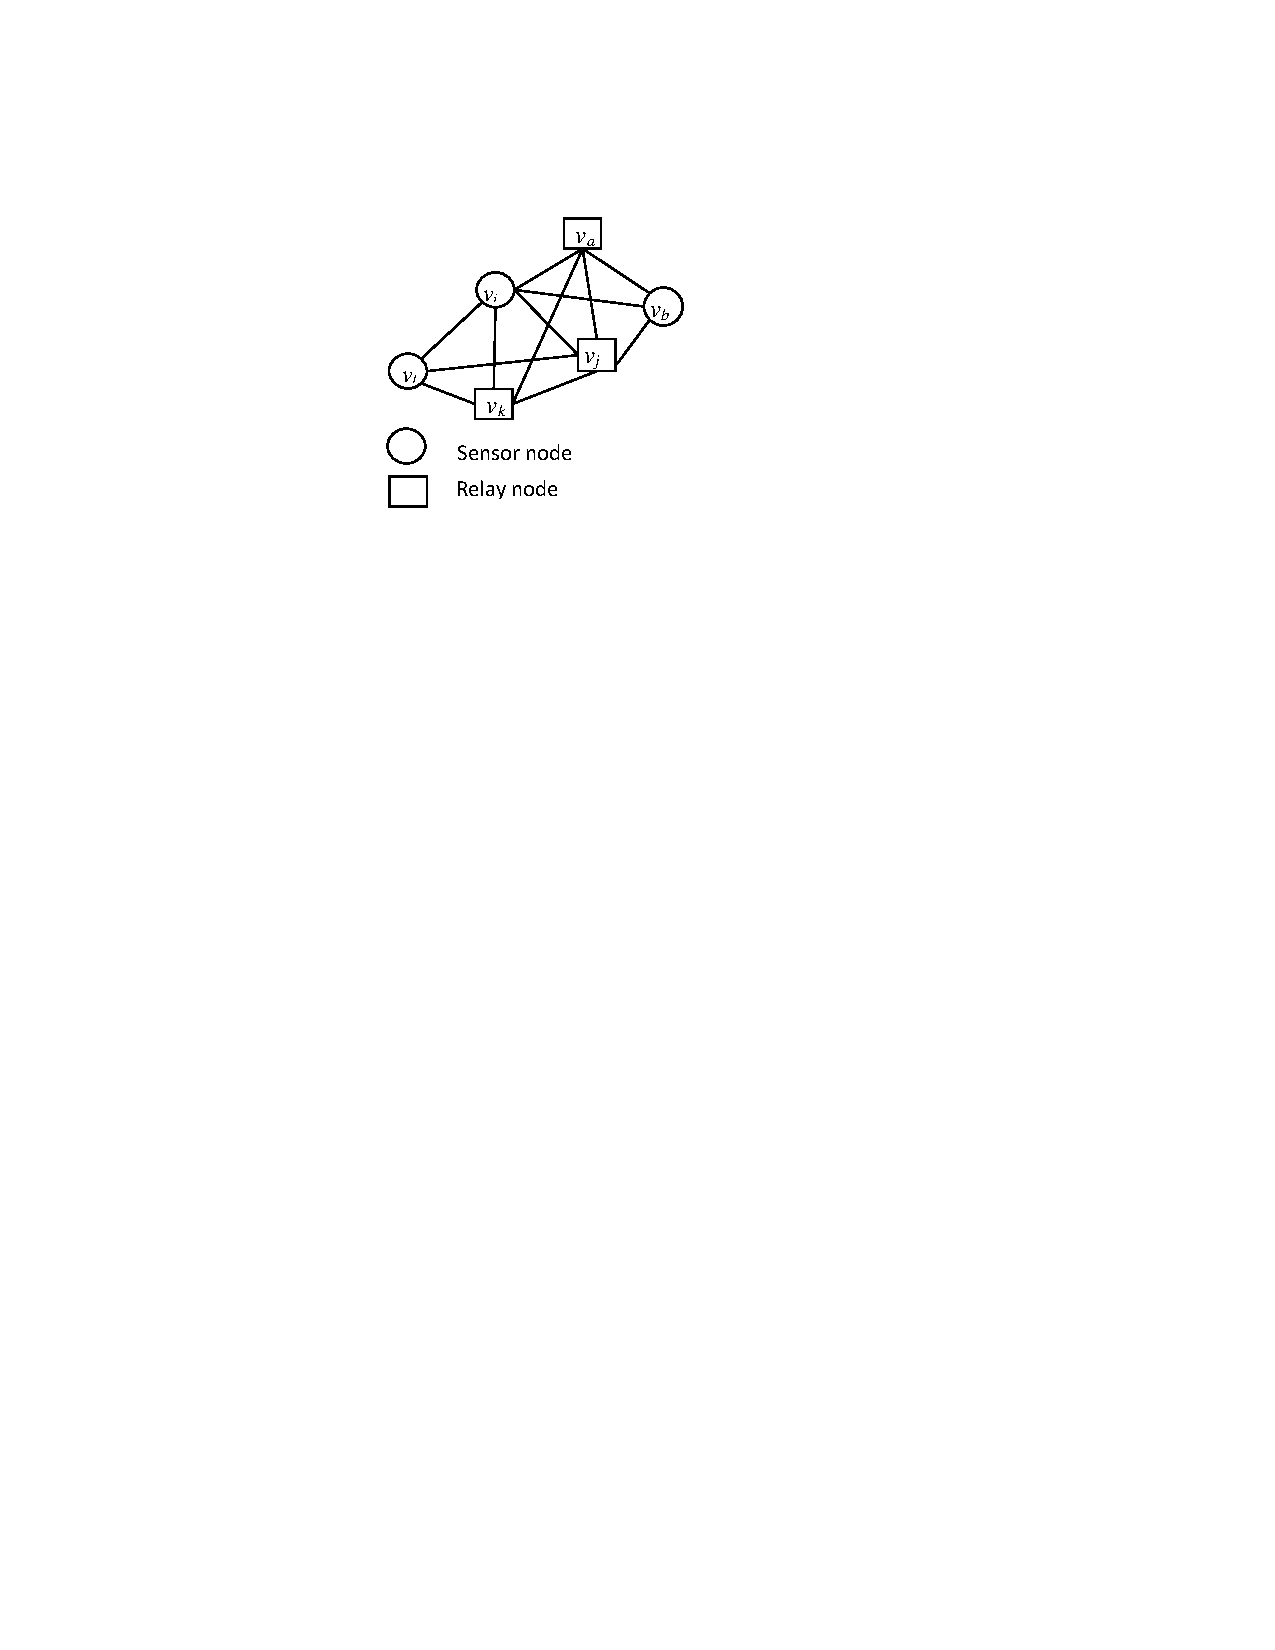
\includegraphics[width=2.2 in, height=1.8 in]{Ch5f3.pdf}
\caption{A 3-tree fragment}
\label{fig:sttype2}
\end{minipage}
\begin{minipage}{0.5\linewidth}
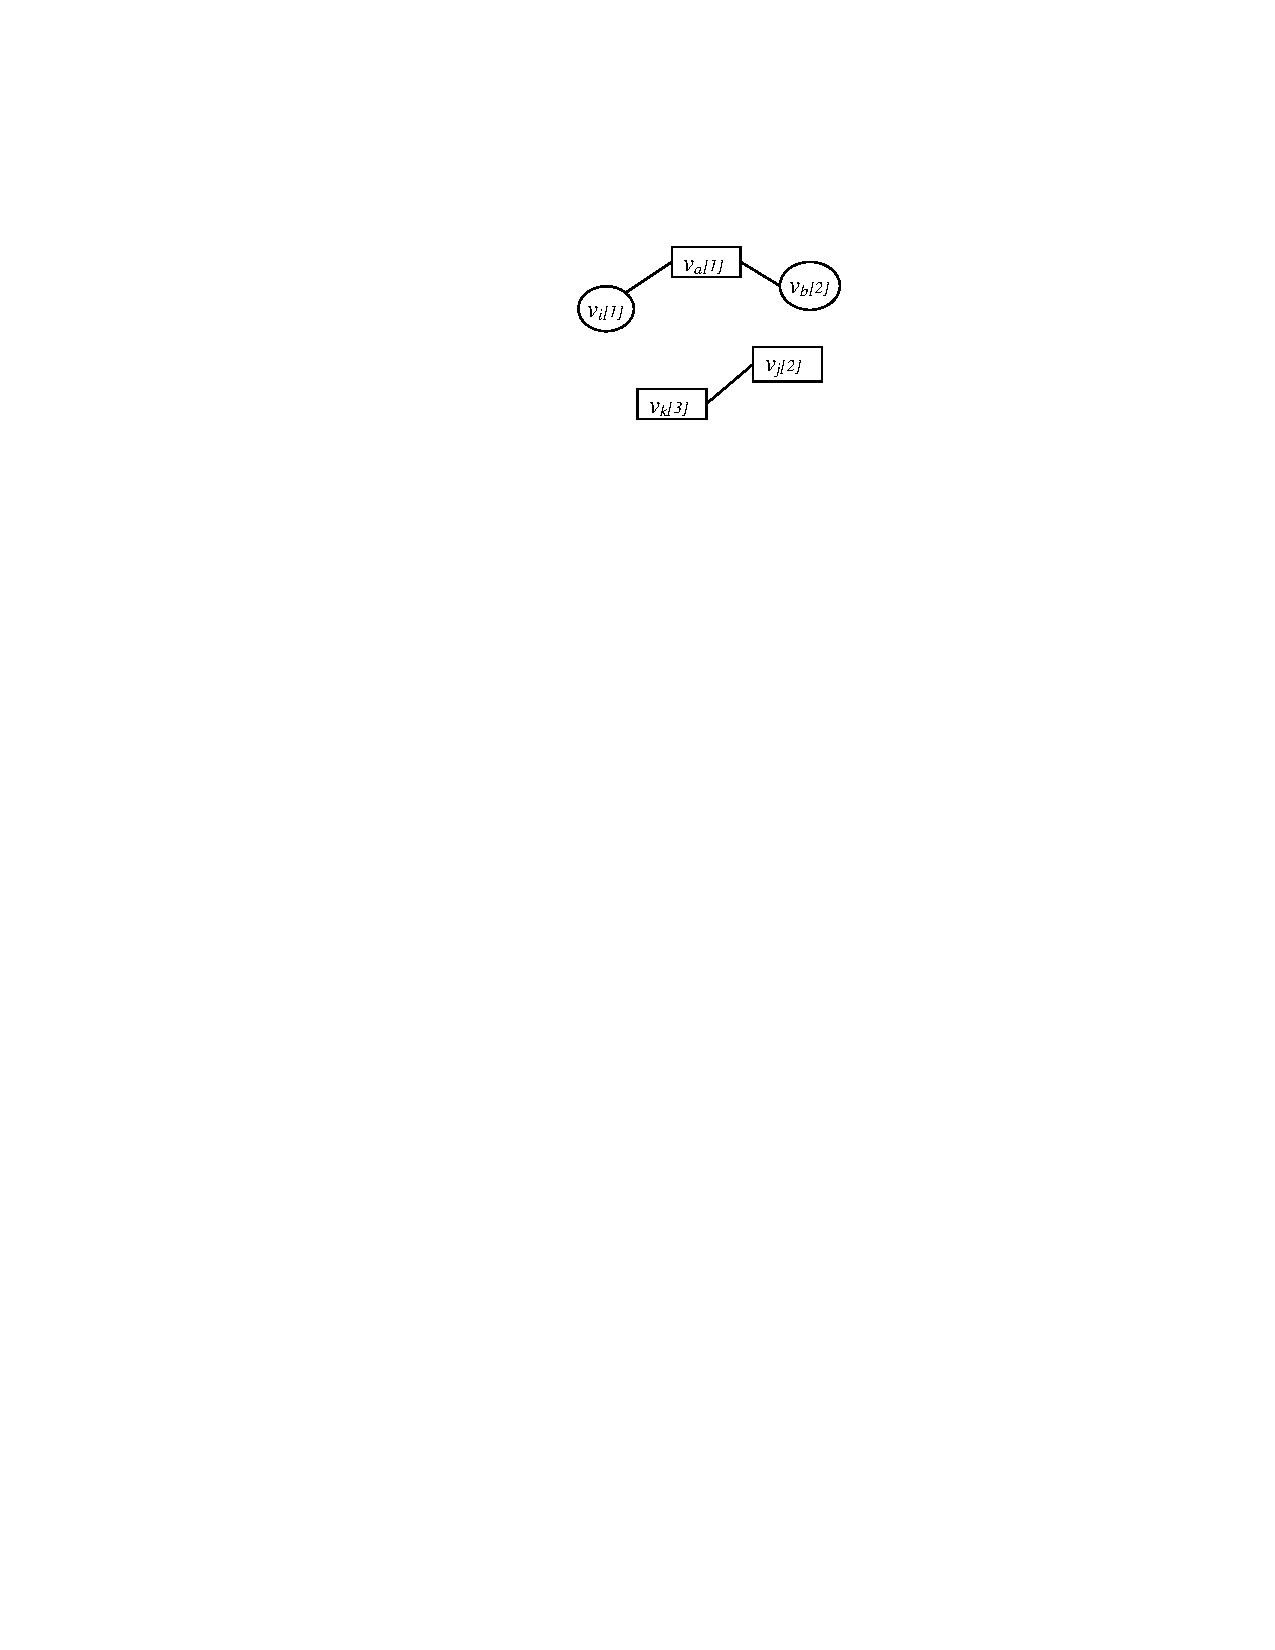
\includegraphics[width=1.7 in, height=1.5 in]{Ch5f3_1.pdf}
\caption{A state $S$ on $\{v_a,v_b,v_i,v_j,v_k\}$}
\label{fig:sttype2_node}
\end{minipage}
\end{figure}
The rationale behind the definition of the $SR\mbox{-}type$ is that when we merge tables containing summary information of two subgraphs $G_1$ and $G_2$ to compute summary information of the union graph $G_1\cup G_2$, we need to know  how many sensor nodes are in each connected component of each state $S$ summarized in the class $SR\mbox{-}type(S)$.


\subsection{Initializing Tables}

Step 1 of function Main initializes a table $T_H$ associates with each $k$-cliques $H$ of the full graph $k$-tree($G$). Our approach here is similar to the one used in Section \ref{subsec:initt}

\subsection{Merging $\SRCONN$ State Types}
\label{subsec:msst}
Using the same notation of section \ref{subsec:mst}, we explain how to process a pair of keys: $key_1\in T_1$ and $key_2\in T_2$, where $T_1$ and $T_2$ are two tables to be merged.

We consider two network states: $S_i, i=1,2,$ where $S_i$ is a network state of the subgraph $G_i$ reduced onto the clique $K_i$, where $key_i=SR\mbox{-}type(S_i)$. Merging $S_1$ and $S_2$ generates $key_{out}=SR\mbox{-}type(S_1\cup S_2)$.

As  with keys of the $A\mbox{-}type$ (or $AR\mbox{-}type$) the union $S_1 \cup S_2$ is possible only if each common node between $S_1$ and $S_2$ takes the same position in both states.

Now, let
\begin{center}
$\begin{array}[t]{l}
SR\mbox{-}type(S_1)=\{X_{i,c(X_i)}^{Loc(X_i)} : i=1,2, \ldots\},\\

SR\mbox{-}type(S_2)=\{Y_{j,c(Y_j)}^{Loc(L_j)} : j=1,2, \ldots\}, \mbox{and}\\
SR\mbox{-}type(S_1\cup S_2)=\{Z_{k,c(Z_k)}^{Loc(Z_k)} : k=1,2, \ldots\}\end{array}$\\
\end{center}

Then 
\begin{itemize}[noitemsep]
\item The partition $\{Z_k:k=1,2,\}$ is generated by applying partition merge to $\{X_i:i=1,2,\ldots\}$ and $\{Y_j:j=1,2,\ldots\}$.
\item If parts $X_i$ and $Y_j$ are merged together into $Z_k$, and the number of common sensor nodes between $X_i$ and $Y_j$ is denoted $n_{ij}$ then\\
\nwline
\centerline{
$c(Z_k)=max(n_{req},c(X_i)+c(Y_j)-n_{ij})$.
	}
\end{itemize}
Similar to the $\ACONN$ algorithm, the probability $p_{out}$ is the product $T_1(key_1) \times T_2(key_2)$ divided by a correction term  $=\prod (p_x(i):x[i] \mbox{ is common between } key_1 \mbox{ and } key_2)$.

\subsection{Bad State Types}
\label{subsec:bst}

Using the same context and notation of section \ref{subsec:rbst}, we define in this section bad $\SRCONN$ state types. For a given node $v_i$ that is processed  in some iteration of the main loop of function Main, the first part of function Main merges all tables $\{T_{v_i,\alpha} :\alpha=1,2, \ldots,k,base\}$ into table $T_{v_i,base}$.

For a state $S$ of $G_{v_i,base}$, let $n_{sense}(S)$ be the number of sensor nodes that can reach the rest of the graph by nodes in the separator clique $K_{v_i,base}$.
Thus, if $SR\mbox{-}type(S)=\{X_{i,c(X_i)}^{Loc(X_i)}: i=1,2, \ldots,r\}$  then
\nwline
\[
 n_{sense}(S) =
  \begin{cases}
   \displaystyle\sum_{X_j\neq\{v_i\}} c(X_j)  & 
   \begin{array}[t]{l}
   \mbox{if node } v_i \mbox{ appears as a singleton in the partition}\\ (X_1,X_2,\ldots,X_r)
    \end{array}\\
   \displaystyle\sum_{j=1,2,\ldots,r}  c(X_j)   & \mbox{ otherwise}
  \end{cases}
\]
\nwline
Now, let us denote by $n_{v_i,base,sense}$ the number of sensor nodes in the  subgraph $G_{v_i,base}$ reduced onto the $k$-clique $K_{v_i,base}$ at the end of the first part of the main loop in function Main. Thus, $|V_{sense}|-n_{v_,base,sense}$ is the number of sensor nodes outside the graph $G_{v_i,base}$.
By definition of operating states of the $\SRCONN$ problem, $SR\mbox{-}type(S)$ is bad if 

\centerline{$n_{sense}(S)+(|V_{sense}|-n_{v_i,base,sense})\leq n_{req}$.}


We recall that the algorithm removes all such bad state types from $T_{v_i,base}$ in step 9 of function Main. Else, if $SR\mbox{-}type(S)$ is good then the algorithm just removes node $v_i$ and its associated position from $SR\mbox{-}type(S)$.

\subsection{Obtaining Final Result}
\label{subsec:ofr1}
Step 11 of function Main computes $Conn(G,n_{req})$ as the sum of all values in the table $T_{v_{n-k},base}$ corresponding to keys of the form \\
\nwline
\centerline{
$\{X_{i,c(X_i)}^{Loc(X_i)} : i=1,2, \ldots\}$}
\nwline
where the partition part that contains the sink node, say $X_1$, has $c(X_1)\geq n_{req}$.

\subsection{Running Time}
\label{subsec:rt1}
As in Chapter 4, $n$ denotes the number of nodes in $G$, $l_{max}$ denotes the maximum number of locations in the locality set of any node, and $B_k$ denote the $k^{th}$ Bell number.
\begin{theorem}\normalfont In the $\SRCONN$ algorithm we have\label{thm:rt1}
\begin{enumerate}
\item The maximum length of any table is $O(B_kl_{max}^kn_{req}^k)$ 
\item The worst case running time is $O(n(B_kl_{max}^kn_{req}^k)^2)$
\end{enumerate}
\end{theorem}

The proof is similar to the proof of the Theorem \ref{thm:runtym} by observing that adding the counters $c(V_i)$ to state types makes the maximum table length as specified in part 1.

\section{$\SRCONN$ Simulation Results}
\label{sec:srconnsim}
The $\SRCONN$ problem is motivated by applications where an UWSN task can be achieved by any subset of sensor nodes connected the sink and has $\textrm{size}\geq n_{req}$ nodes, where $n_{req}$ is a design parameter.
For such applications, a designer has at least 3 options to achieve a minimum required $Conn(G,n_{req})$ value:

\begin{itemize}
\item tuning the $n_{req}$ parameter,
\item tuning node transmission range $R_{tr}$, and
\item tuning the number of deployed relay nodes.
\end{itemize}
In this section we explore the use of our devised $\SRCONN$ algorithm to tackle such design problem.


\textbf{Test Networks:} As in section \ref{sec:arconnsim}, we use network $G_{10}$ in figure \ref{fig:netI1} and $G_{10,3}$ in figure \ref{fig:netIR}


\textbf{Effect of varying $n_{req}$:} Figure \ref{Fig:CvCwr1} illustrates the achieved $Conn(G,n_{req})$ as $n_{req}$ varies in the range $[1,10]$. Figure \ref{Fig:CvCwr2} illustrates the achieved $Conn(G,n_{req})$ as $n_{req}$ varies in the range $[1,10]$, and $R_{tr}$ varies in the range $[2.5,5.5]$.

\begin{figure}[!htb]
\begin{minipage}{0.5\linewidth}
\centering
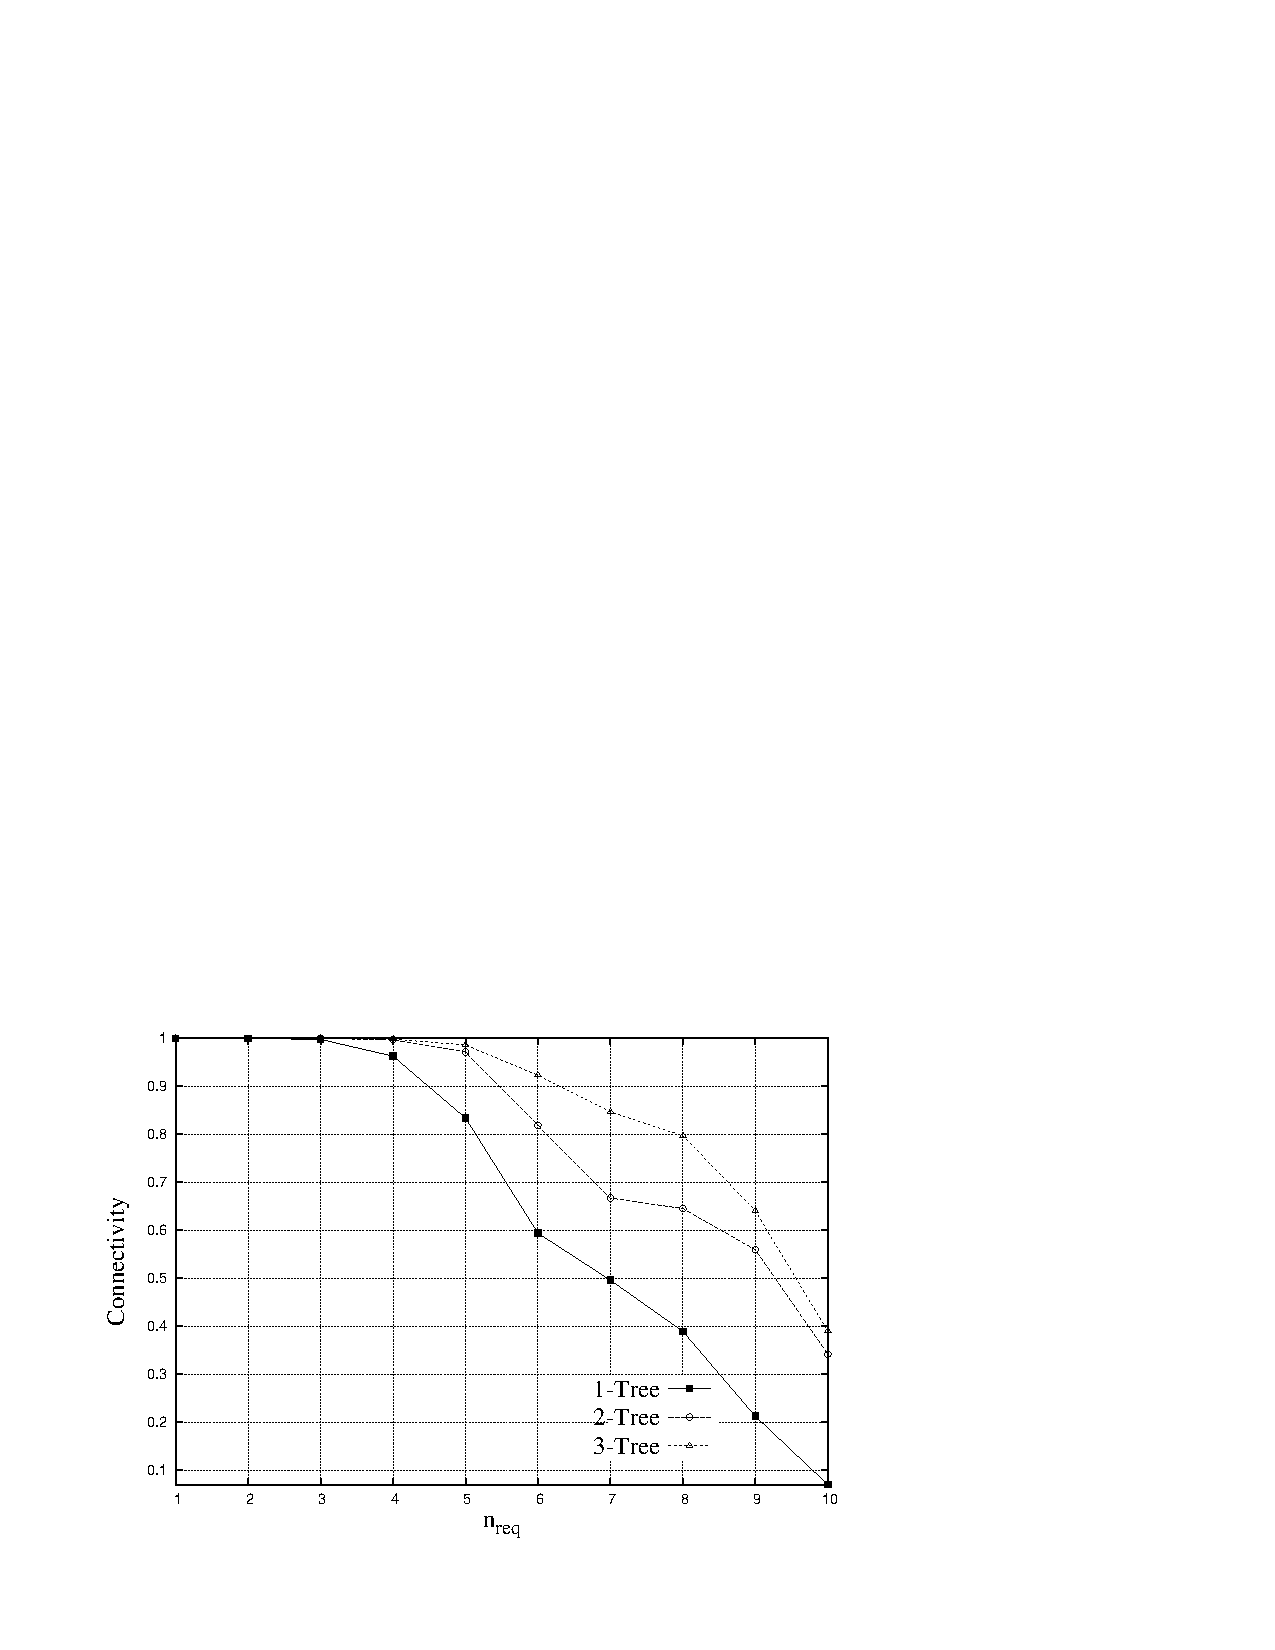
\includegraphics[width=3 in, height=2.4 in]{abc.pdf}
\caption{Connectivity versus $n_{req}$}
\label{Fig:CvCwr1}
\end{minipage}
\begin{minipage}{0.5\linewidth}
\centering
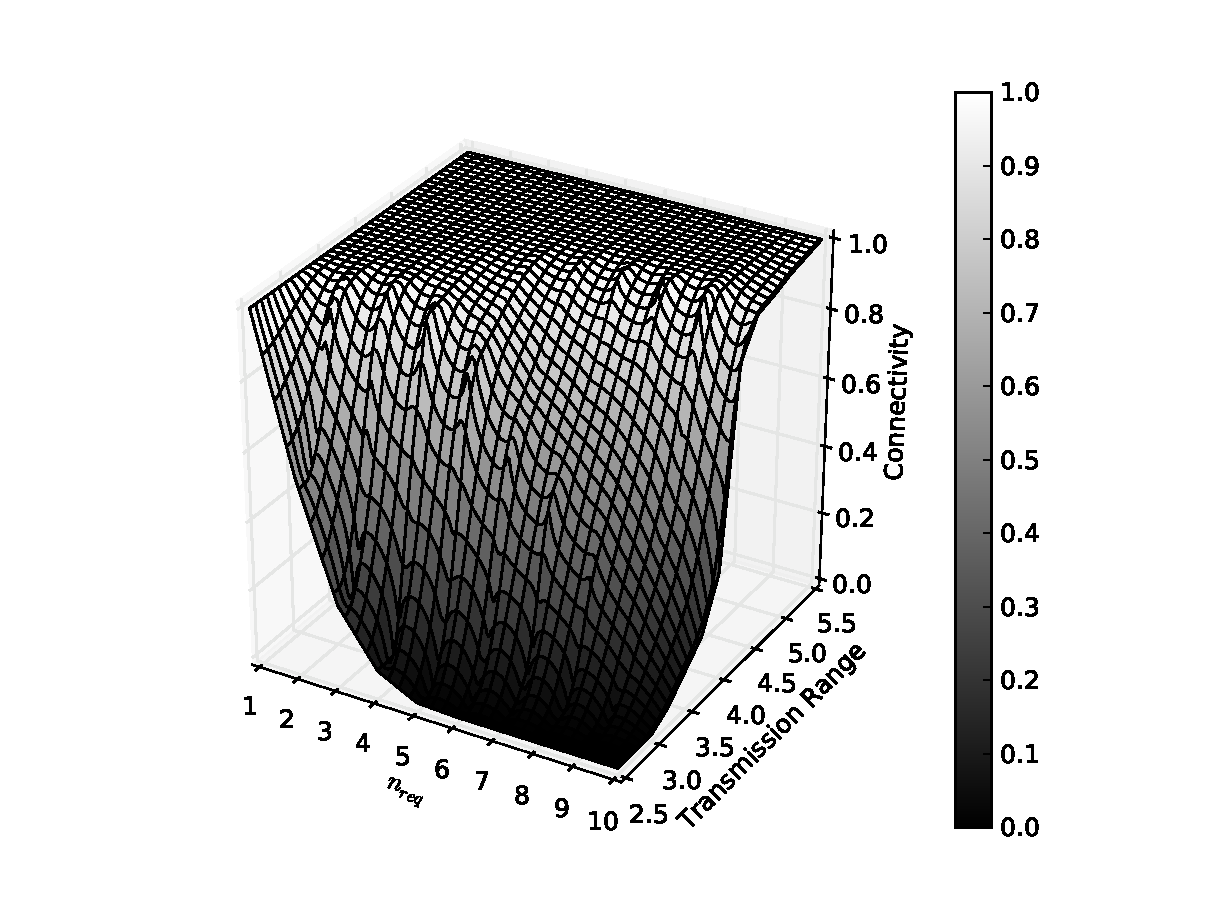
\includegraphics[width=3 in, height=2.4 in]{3D.pdf}
\caption{Connectivity versus $n_{req}$ and transmission range}
\label{Fig:CvCwr2}
\end{minipage}
\end{figure}

\section{Concluding Remarks}
In this chapter we have presented extensions to the $\ACONN$ dynamic programming algorithm. The extensions yield two algorithms for solving the $\ARCONN$ and $\SRCONN$ problem on partial $k$-trees where a $k$-$PES$ is specified for each problem instance. The algorithms run in polynomial time on any partial $k$-tree with fixed $k$. The algorithms are implemented in $C\mbox{++}$ and provide network design tools for analyzing probabilistic connectivity when any combination of the following parameters change: node locality sets and their probabilistic distribution, node transmission range, number of relay nodes that can be deployed, and the number of nodes connected to the sink required achieve a given task.  
